\documentclass[12pt]{article} % Default font size is 12pt, it can be changed here
\usepackage{fontspec}
%Ligatures=TexOff disable the Tex specific ligatures which converst quotes into typographic quotes
\setmainfont{OpenSans}[Ligatures=TeXOff, Path=fonts/,Extension=.ttf, UprightFont=*-Regular, ItalicFont=*-Italic, BoldFont=*-Bold, BoldItalicFont=*-BoldItalic]
\usepackage{microtype}

%\usepackage{tabulary}
\usepackage{tabu} %span tables over multiple pages while still wrapping text inside cells
\usepackage{longtable} %needed by tabu package
\usepackage{geometry}
\geometry{a4paper, total={170mm,257mm}, left=20mm, top=20mm, }

\usepackage{graphicx} % Required for including pictures
\usepackage{tikz}
\usepackage{float} % Allows putting an [H] in \begin{figure} to specify the exact location of the figure
\usepackage{wrapfig} % Allows in-line images such as the example fish picture
\usepackage{lipsum} % Used for inserting dummy 'Lorem ipsum' text into the template

\newcommand{\sectionbreak}{\clearpage}

\graphicspath{{../graphics/}} % Specifies the directory where pictures are stored 

\usepackage{tcolorbox}
\tcbuselibrary{skins}

\usepackage{listings} % Code listings
\usepackage{color}
\definecolor{lightgray}{rgb}{.9,.9,.9}
\definecolor{darkgray}{rgb}{.4,.4,.4}
\definecolor{purple}{rgb}{0.65, 0.12, 0.82}
\definecolor{orange}{rgb}{1, 0.4, 0.0}

\lstdefinelanguage{JavaScript}{
  keywords={typeof, new, true, false, catch, function, return, null, catch, switch, var, if, in, while, do, else, case, break},
  keywordstyle=\color{blue}\bfseries,
  ndkeywords={class, export, boolean, throw, implements, import, this},
  ndkeywordstyle=\color{darkgray}\bfseries,
  identifierstyle=\color{black},
  sensitive=false,
  comment=[l]{//},
  morecomment=[s]{/*}{*/},
  commentstyle=\color{orange}\ttfamily,
  stringstyle=\color{purple}\ttfamily,
  morestring=[b]',
  morestring=[b]"
}

\lstset{
   language=JavaScript,
   backgroundcolor=\color{blue!5},
   extendedchars=true,
   basicstyle=\scriptsize\ttfamily,
   showstringspaces=false,
   showspaces=false,
   tabsize=4,
   breaklines=true,
   showtabs=false,
   captionpos=b,
   frame=leftline,
   rulecolor=\color{blue!20},
   framerule=2pt
}
\setlength{\parindent}{0pt} % removes the default indentation of first lines
\setlength{\tabcolsep}{12pt}

\NewEnviron{squeeze}{\scalebox{.9}[1.0]{\BODY}}
\NewEnviron{squeezealot}{\scalebox{.8}[1.0]{\BODY}}

\newenvironment{mono}{\ttfamily}{\par}
\newenvironment{keyword}{\leavevmode\color{magenta}}{}
\newenvironment{keywordpurple}{\leavevmode\color{purple}}{}
\newenvironment{examplecomment}{\leavevmode\color{magenta!60!white}}{}
\newenvironment{code}{\begin{mdframed}[linewidth=4pt, linecolor=blue!40, topline=false, bottomline=false, rightline=false, backgroundcolor=blue!10]\begin{mono}}{\end{mono}\end{mdframed}}

\newenvironment{properties}
	{
    	\footnotesize\renewcommand{\arraystretch}{1.30}
  		\renewcommand{\tabcolsep}{0pt}
   		\begin{longtable}{>{\begin{keyword}}p{3.1cm}<{\end{keyword}}p{13.9cm}}
    	\hline
	}
	{
		\hline\end{longtable}\vspace{5mm}
	}
	
\newenvironment{parameters}
	{
    	\footnotesize\renewcommand{\arraystretch}{1.30}
    	\renewcommand{\tabcolsep}{0pt}
 		\begin{longtable}{>{\begin{keyword}}p{3cm}<{\end{keyword}}>{\begin{em}}p{1.5cm}<{\end{em}}p{12.5cm}}
    	\hline
	}
	{
		\hline\end{longtable}\scriptsize\vspace{-5mm}*mandatory parameters\vspace{5mm}
	}
	
\newtcolorbox{exampleResultBox}[2][]{
	skin=bicolor,colback=magenta!10!white,
	fonttitle=\bfseries,
	colbacktitle=magenta,
	bottomtitle=2mm,
	toptitle=2mm,
	colbacklower=black!10!white,
	title=#2,#1,
	boxrule=0mm,
	middle=0mm,
	boxsep=0mm,
	left=5mm,
	right=5mm,
	bottom=5mm,
	top=5mm,
	after upper={\hyphenpenalty=10000\raggedright\vskip 5mm\null},
	subtitle style={colback=black,left=5mm,right=5mm,bottom=2mm,top=2mm}
}

\newtcolorbox{exampleBox}[2][]{
	colback=magenta!10!white,
	fonttitle=\bfseries,
	colbacktitle=magenta,
	boxrule=0mm,
	title=#2,#1
}

\newtcolorbox{resultBox}[2][]{
	colback=black!20!white,
	fonttitle=\bfseries,
	colbacktitle=black,
	boxrule=0mm,
	title=#2,#1
}

\newtcolorbox{advancedBox}[2][]{
	colback=purple!10!white,
	fonttitle=\bfseries,
	colbacktitle=purple,
	boxrule=0mm,
	title=#2,#1
}

	
\setlength{\parskip}{0.5em}

\DeclareTextFontCommand{\kw}{\keyword}
\DeclareTextFontCommand{\kwp}{\keywordpurple}

\begin{document}
\small

%----------------------------------------------------------------------------------------
%	TITLE PAGE
%----------------------------------------------------------------------------------------

\begin{titlepage}

\newcommand{\HRule}{\rule{\linewidth}{0.5mm}} % Defines a new command for the horizontal lines, change thickness here

\center % Center everything on the page

\begin{tikzpicture}[remember picture,overlay]
   \node[anchor=north west,inner sep=1cm] at (current page.north west){
\includegraphics[width=3cm]{logos/UniLogo}};
\end{tikzpicture}

\begin{tikzpicture}[remember picture,overlay]
   \node[anchor=north east,inner sep=1cm] at (current page.north east){
\includegraphics[width=6cm]{logos/LUCET}};
\end{tikzpicture}\\[6cm]

\textsc{\large OASYS v3.6.0}\\[0.5cm] % Software version this document applies to

\HRule \\[0.4cm]
{ \huge \bfseries Advanced Editor Keyword Reference}\\[0.4cm] % Title of document
\HRule \\[1.5cm]

\large
\textit{Author:} Eric J. FRANCOIS % Your name
\begin{tikzpicture}[remember picture,overlay]
   \node[anchor=south,inner sep=2cm] at (current page.south){\large \today};
\end{tikzpicture}

\end{titlepage}

\newpage

\section{description}\label{sec:description}

OASYS uses proprietary keywords in order to define input fields with specific attributes that allow to customise these input fields to the users' needs.
Some keywords also exist for other purposes, like advanced layouting.
\subsection{structure of a keyword}\label{subsec:structure-of-a-keyword}
Every keyword follows the same syntactical rules:
\begin{itemize}
\item every keyword needs the opening and closing brackets \kw{[@ ... @]}
\item the keyword follows the opening bracket without space, e.g. \kw{[@TF ... @]}
\item every keyword can have a multitude of attributes
\item attributes can take 2 forms:\begin{itemize}
	\item[] \kw{ATTRIBUTE="..."} for attributes with a value
	\item[] \kw{ATTRIBUTE} for attributes that take effect merely by being present
\end{itemize}
\item attributes can be written in any order
\item all fields can take the attribute \kw{OPTIONAL} if a field is not mandatory
\item all fields can take an \kw{EXPORT} attribute, which exports the value of the field to a global variable that can be used in overviews or scripts.
If the \kw{EXPORT} keyword does not take a value, the variable will have the same name as the ID resp.
GROUP of the field being exported.
If another name is required (e.g.\ if fields in different pages carry the same ID) then the attribute must have a value which designates the variable name: \kw{EXPORT="var\_01"}
\item all fields can take a \kw{COMMENT="…"} attribute which does not have any influence on the content.
It's used only to store additional information which can later be exported via a dedicated API\@.
\end{itemize}
\newpage

\section{scoring}\label{sec:scoring}

OASYS allows some types of answers to be automatically graded.
This is commonly the case for closed answer formats such as single or multiple choice questions.
Under certain conditions it also makes sense to automatically grade textfields, if a very specific word is expected (e.g.\ vocabulary checks or grammar tests). \\

But automatically checking whether a question is correct or not is not enough.
The test creator is also required to tell OASYS how many points to attribute to which question.
Also sometimes not responding to a question is graded less harshly then giving a wrong answer. \\

In general there are 2 approaches to scoring—by adding points or by substracting points: 

\subsection{adding points}\label{subsec:adding-points}
In this case we start out with 0 points and for every correct answer a certain amount of points are added.
Sometimes a missing answer will get a smaller amount of points (e.g.\ 5 points for a correct answer, 2 points for a missing answer and of course no points for a wrong answer).

\subsection{substracting points}\label{subsec:substracting-points}
In this model we start out with a given amount of points, and for every error we substract a certain amount of points.
In analogy to the previous example, we would give 5 initial points, 0 for a correct answer, -3 for a missing answer and -5 for a wrong answer.\\

The advantage of this system plays when working with multiple choice questions.
For instance there are 6 possible choices to check, 3 of which are correct.
If 2 correct ones are selected but one is missing, the score will be 3 out of 5, while if only 1 correct answer is given and 2 are missing 2 * 3 points would be substracted (with 0 points being the lowest possible score) giving 0 points.

\subsection{defining the score}\label{subsec:defining-the-score}

In autograding mode we need to set 4 numbers for points to attribute.
This is done with the SCORE attribute and the numbers to be given are done so in the following order:  initial, correct, wrong and missing:

\begin{exampleBox}{Example}
To give 5 points for a correct answer and 2 to a missing answer the attribute would look like this:\\

\kw{SCORE="0 5 0 2"}\\

However to give 5 initial points and substract 5 for a wrong answer and 3 for a missing answer, the attributes takes the following form: \\

\kw{SCORE="5 0 -5 -3"}

\end{exampleBox}
\vspace{0.5cm}

The \kw{SCORE} attribute is available in all field types and is not mentioned specifically in every field description and attribute list.

\newpage

\section{available keywords}\label{sec:available-keywords}

Here is the list of currently defined keywords in OASYS. Some keywords that are still in development or being beta tested are not included, as they are subject to change.

\subsection{text field}\label{subsec:text-field}

Syntax:\hspace{0.5cm}\kw{[@TF ... @]}

\begin{properties}
ID & this defines the variable name for the results of the text field;
if omitted, the fields will be autonamed: tf\_1, tf\_2, \ldots etc.\\
WIDTH & width of the field as CSS string, if only a number is given the unit defaults to pixels [default: \kw{200}]\\
MAXWIDTH & maximum width as CSS string which overrides the width if field becomes too large [default: \kw{calc(100\% - 25px)}]\\
ALIGN & text alignment;
possible values: \kw{left}, \kw{center}, \kw{right} [default: \kw{left}]\\
PATTERN & a regular expression that defines what can be entered in the field;
for a field that can accept decimal numbers only, use the following: \newline \kw{PATTERN="\string^\string\-?(\string\d*[.,])?\string\d*\$"} \\
CORRECT & the expected value for this text field (for auto correction) \\
IGNORECASE & if this is present the auto corrector will ignore case \\
PREFILL & a value to prefill the text field with \\
READONLY & make the text field uneditable (usually used with a prefilled value as example of a task to do) \\
PLACEHOLDER & placeholder text to show in text field as long has nothing as been typed into it \\
\end{properties}
\vspace{0.1cm}

A textfield without attributes \kw{[@TF@]} would be 200 pixels wide, left aligned and called tf\_1.

\begin{exampleBox}{Example}
A text field that accepts numbers only, 50 pixels wide, center aligned and with the name "salary":\\

\kw{[@TF ID="salary" WIDTH="50" ALIGN="center" PATTERN="\string^\string\-?(\string\d*[.,])?\string\d*\$" @]}
\end{exampleBox}
	
When defining auto correction more than one acceptable answer can be defined by separating the correct answers with a pipe symbol: |\\

Also beware that auto correction does not take into account the language in which an answer is given, because the test language can be changed while the test is running.
It is mandatory that the correct answer from all languages of the test are defined as correct.
The \kw{CORRECT} attribute with its values most be given identically in all languages to be correctly recognized.

\begin{exampleBox}{Example}
Here the English and German version of a word are recognized as correct:\\

\kw{[@TF ID="negativeParticle" WIDTH="50" CORRECT="electron|Elektron" @]}
\end{exampleBox}

	
\subsection{text area}\label{subsec:text-area}

Syntax:\hspace{0.5cm}\kw{[@TA ... @]}

\begin{properties}
\hline
ID & this defines the variable name for the results of the text area;
if omitted, the fields will be autonamed: ta\_1, ta\_2, \ldots etc.\\
WIDTH & width of the area (in pixels) [default: \kw{990}]\\
MAXWIDTH & maximum width as CSS string which overrides the width if field becomes too large [default: \kw{calc(100\% - 25px)}]\\
HEIGHT & height of the area (in pixels) [default: \kw{200}]\\
ALIGN & text alignment;
possible values: \kw{left}, \kw{center}, \kw{right} [default: \kw{left}]\\
PREFILL & a value to prefill the text field with \\
READONLY & make the text field uneditable (usually used with a prefilled value as example of a task to do) \\
PLACEHOLDER & placeholder text to show in text field as long has nothing as been typed into it \\
RESIZE & defines if the user may resize the text area; \newline possible values: \kw{horizontal}, \kw{vertical}, \kw{both}, \kw{none} [default: \kw{none}] \\
\hline
\end{properties}
\vspace{0.1cm}

\begin{exampleBox}{Example}
	A text area that is not mandatory, 600 pixels wide, 400 pixels heigh, left aligned and with the name "comments": \\
	\kw{[@TA ID="comments" WIDTH="600" HEIGHT="400" OPTIONAL@]}
\end{exampleBox}

\subsection{drop down list}\label{subsec:drop-down-list}

Syntax:\hspace{0.5cm}\kw{[@DD ... @]}

\begin{properties}
\hline
ID & this defines the variable name for the results of the drop down list;
if omitted, the fields will be autonamed: dd\_1, dd\_2, \ldots etc.\\
WIDTH & width of the drop down list (in pixels) [default: \kw{200}]\\
OPTIONS & the list of options the test taker can choose from, separated with a vertical bar (pipe)\\
\hline
\end{properties}
\vspace{0.1cm}

\begin{exampleBox}{Example}
	A field of gender choice could look like this:\\
	\kw{[@DD WIDTH="150" OPTIONS="female|male|transgender"@]}
\end{exampleBox}

The answers given by test takers are reported by a number representing the number of the choice from the list.
Once data collection has started, it is imperative to not change the order of the choices or add resp.
remove a choice from the list, otherwise the data given already will be corrupted.\\

When using a drop down in more than one language, the order of the options must be the same in all languages, otherwise the numbers given in one language correspond to the wrong answer in another language.
A common mistake here would be to ask for nationality and try to alphabetize the list in every language.
While the order would be "English, French, German" in English, the order changes to "Deutsch, Englisch, Französisch" in German.
So when replying "German" in English, the number would be 3 which will then be interpreted as "Französisch" when switching to the German version.
If alphabetical order is relevant, please use the choice interaction in OASYS' graphical user interface, rather than the advanced editor to do this. \\

In order to mark an answer in a drop down list as being correct (for the sake of auto correction), an asterisk is to be added immediately after the label.
Since a drop down list is a single choice field, only one answer must be marked as correct.
The corresponding answer must be marked as correct in every language of the field.\\

\begin{exampleBox}{Example}
	Which particle of an atom has a negative charge?\\
	\kw{[@DD ID="negativeParticle" WIDTH="150" OPTIONS="electron*|neutron|proton"@]}
\end{exampleBox}

\subsection{radio buttons}\label{subsec:radio-buttons}

Syntax:\hspace{0.5cm}\kw{[@RB ... @]} \\

Radio buttons allow the user to choose exactly one out of a group of several options.
If a new option is selected the previously active one will be cleared again.
By default radio buttons are round, which allows to distnguish them from checkboxes (see below).
Once a radio button has been selected, it is impossible to clear the group again entirely.

\begin{properties}
\hline
GROUP & this defines the variable name for the results of a group of radio buttons;
if omitted, the groups will be autonamed: rb\_1, rb\_2, \ldots (c.f. \kw{NG} keyword) \\
VALUE & this is the value of an individual button within the group;
the variable defined with \kw{GROUP} will get this value when it is selected;
if omitted, the values will be increasing numbers in order of occurrence \\
NG & if no \kw{GROUP} is defined, using the autonaming feature, this keyword tells the parser to start a new group;
the very first group does not need \kw{NG}\\
HEIGHT & if there is necessity of bigger radio buttons (e.g.\ for accessibility reasons or for touch devices), the \kw{HEIGHT} keyword takes a value in pixels for the diameter of the radio button. \\
CORRECT & if present this attribute indicates that this is the expected answer in this radio button group;
alternatively to the \kw{CORRECT} attribute it's possible to add an asterisk after the keyword: \kw{[@RB* ... @]} \\
NOREPLY & if present, this attribute marks this answer as identical to not replying at all to this group—that is only relevant when working with a scoring model where no answer is scored differently from wrong answers. \\
\hline
\end{properties}
\vspace{0.1cm}

When a \kw{GROUP} is defined, it will be applied for all following radio buttons until a new \kw{GROUP} or an \kw{NG} keyword is encountered.

In the same manner, the \kw{HEIGHT} keyword will stick for any following radio buttons, until a new \kw{HEIGHT} is set.
By default, it will be set at the very first radio button, and from there it will remain unchanged until the end of the item, over all the groups.
The height value always applies to the whole group;
it is impossible to create radio buttons of different sizes within a single group.\\

\begin{exampleBox}{Example of auto corrected radio buttons}
	Which particle of an atom has a negative charge?\\
	\kw{[@RB* GROUP="negativeParticle" VALUE="electron"@]} electron\\
	\kw{[@RB VALUE="neutron"@]} neutron\\
	\kw{[@RB VALUE="proton"@]} proton\\
	\kw{[@RB VALUE="dontknow" NOREPLY @]} I don't know
\end{exampleBox}

\vspace{1cm}

\begin{exampleResultBox}{Example with automatically named radio buttons:}
\begin{tabular}{p{0.45\textwidth} p{0.45\textwidth}}
	What is your gender: & \examplecomment{default values}\\
\kw{[@RB@]} female & \examplecomment{group="rb\_1" value="1"}\\
\kw{[@RB@]} male & \examplecomment{group="rb\_1" value="2"}\\
\kw{[@RB@]} transgender & \examplecomment{group="rb\_1" value="3"}\\
& \\
What is your marital status: &\\
\kw{[@RB NG@]} single & \examplecomment{group="rb\_2" value="1"}\\
\kw{[@RB@]} married & \examplecomment{group="rb\_2" value="2"}\\
\kw{[@RB@]} widowed & \examplecomment{group="rb\_2" value="3"}\\

\end{tabular}
\tcblower
\tcbsubtitle{The results of a single man would look like this:}
	\begin{tabular}{l|l}
		\textbf{variable} & \textbf{value} \\
		\hline
		rb\_1 & 2\\
		rb\_2 & 1\\
	\end{tabular}
\end{exampleResultBox}

\vspace{1cm}

\begin{exampleResultBox}{The same example again with manual naming:}
What is your gender: \\
\kw{[@RB GROUP="gender" VALUE="F"@]} female\\
\kw{[@RB VALUE="M"@]} male \\
\kw{[@RB VALUE="T"@]} transgender \\
\\
What is your marital status:\\
\kw{[@RB GROUP="status" VALUE="single"@]} single\\
\kw{[@RB VALUE="married"@]} married\\
\kw{[@RB VALUE="widowed"@]} widowed
\tcblower
\tcbsubtitle{The results of a single man would look like this:}
\begin{tabular}{l|l}
\textbf{variable} & \textbf{value} \\
\hline
gender & M\\
status & single\\
\end{tabular}
\end{exampleResultBox}

\subsection{checkboxes}\label{subsec:checkboxes}

Syntax:\hspace{0.5cm}\kw{[@CB ... @]} \\

Checkboxes allow the user to choose any number of choices from a group of options.
This is the typical answer format for questions like "check all that apply".
By default checkboxes are square and get a checkmark inside when selected.
Selected options can be cleared again by clicking on the checkbox once more.

\begin{properties}
\hline
GROUP & this defines the variable name for the results of a group of checkboxes;
if omitted, the groups will be autonamed: cb\_1, cb\_2, \ldots (c.f. \kw{NG} keyword) \\
VALUE & this is the value of an individual box within the group;
the variable defined with \kw{GROUP} will be an enumeration of the values of all checked boxes;
if omitted, the values will be increasing numbers in order of occurrence \\
NG & if no \kw{GROUP} is defined, using the autonaming feature, this keyword tells the parser to start a new group;
the very first group does not need \kw{NG}\\
HEIGHT & if there is necessity of bigger checkboxes (e.g.\ for accessibility reasons or for touch devices), the \kw{HEIGHT} keyword takes a value in pixels for the diameter of the checkbox \\
CORRECT & if present this attribute indicates that this is part of the expected answer in this checkbox group;
alternatively to the \kw{CORRECT} attribute it's possible to add an asterisk after the keyword: \kw{[@CB* ... @]} \\
MAX & this number limits the number of answers possible in the group—while the default behaviour is that all checkboxes in a group can be selected, it's possible to artificially limit that.
This may be useful in elections where, for instance, 2 candidates out of 10 may be selected. \\
RULE & this defines what is the number of expected answers.
This influences the colouring of the button—if supported by the selected skin—to show if a question has been filled in completely.
If the "limit navigation" option is active in the test this setting informs if a test taker can proceed to the next page or not.
The syntax is as follows: for "2 or less" it's possible to write either \kw{<3} or \kw{2-}, for "3 or more" it's possible to write \kw{>2} or \kw{3+} and "anything from 2 to 4" is written \kw{2..4} \\
\hline
\end{properties}
\vspace{0.1cm}

When a \kw{GROUP} is defined, it will be applied for all following checkboxes until a new \kw{GROUP} or an NG keyword is encountered.

In the same manner, the \kw{HEIGHT} keyword will stick for any following checkboxes, until a new \kw{HEIGHT} is set.
By default, it will be set at the very first checkboxes, and from there it will remain unchanged until the end of the item, over all the groups.

\vspace{0.5cm}

\begin{exampleBox}{Example of auto corrected checkboxes}
	Which particles of an atom have a charge (negative or positive)?\\
	\kw{[@CB* GROUP="negativeParticle" VALUE="electron"@]} electron\\
	\kw{[@CB VALUE="neutron"@]} neutron\\
	\kw{[@CB* VALUE="proton"@]} proton
\end{exampleBox}

\vspace{1cm}

\begin{exampleResultBox}{Example with automatically named checkboxes:}
\begin{tabular}{p{0.45\textwidth} p{0.45\textwidth}}
What kind of food do you like:& \examplecomment{default values}\\
\kw{[@CB@]} meat & \examplecomment{group="cb\_1" value="1"}\\
\kw{[@CB@]} seafood & \examplecomment{group="cb\_1" value="2"}\\
\kw{[@CB@]} vegetables & \examplecomment{group="cb\_1" value="3"}\\
\kw{[@CB@]} fruit & \examplecomment{group="cb\_1" value="4"}\\
\kw{[@CB@]} bread & \examplecomment{group="cb\_1" value="5"}\\
\kw{[@CB@]} sweets & \examplecomment{group="cb\_1" value="6"}
\end{tabular}
\tcblower
\tcbsubtitle{The results of a vegetarian might look like this:}
\begin{tabular}{l|l}
\textbf{variable} & \textbf{value} \\
\hline
cb\_1 & ["3","4","5","6"]\\
\end{tabular}
\end{exampleResultBox}

\begin{exampleResultBox}{The same example again with manual naming:}
What kind of food do you like:\\
\kw{[@CB GROUP="food" VALUE="meat"@]} meat\\
\kw{[@CB VALUE="seafood"@]} seafood\\
\kw{[@CB VALUE="vegetables"@]} vegetables \\
\kw{[@CB VALUE="fruit"@]} fruit\\
\kw{[@CB VALUE="bread"@]} bread\\
\kw{[@CB VALUE="sweets"@]} sweets
\tcblower
\tcbsubtitle{The results of the same vegetarian as above would now read as follows:}
\begin{tabular}{l|l}
\textbf{variable} & \textbf{value} \\
\hline
food & ["vegetables","fruit","bread","sweets"]\\
\end{tabular}
\end{exampleResultBox}
\subsection{label}\label{subsec:label}

Syntax:\hspace{0.5cm}\kw{[@LB ... @]}some text\kw{[@/LB@]}

When using checkboxes or radio buttons, you would like the test takers to be able to click on the label accompanying the checkbox or radio button.
On a touch device this is all the more important.

The label keyword defines which part should be clickable.
The keyword consists of an opening and a closing tag—everything in-between will be clickable.
The label can also be used for text fields and text areas.
In that case the field gets focused when the test taker clicks on the label.

\begin{properties}
\hline
TYPE & this defines the type of element the label is trying to attach to: "\kw{RB}" for radio buttons, "\kw{CB}" for checkboxes, "\kw{TF}" for text fields and "\kw{TA}" for text areas.
You can also define "\kw{*}" as type which will apply it to either checkbox or radio button but ignore text related fields.
The "\kw{*}" is the default setting, hence the \kw{TYPE} must always be specified if linking to a text field or area.\\
LINK & this links the label to a specific group or field—in general this can be left out, as OASYS links the labels in order of occurrence automatically.
If used, the value must be identical to the \kw{GROUP} value or in case of a text field or area it must match the \kw{ID} of that field.\\
\hline
\end{properties}
\vspace{0.1cm}

Our previous checkbox example combined with labels will look like this:
\begin{exampleBox}{Example}
What kind of food do you like:\\
\kw{[@CB GROUP="food" VALUE="meat"@] [@LB@]}meat\kw{[@/LB@]}\\
\kw{[@CB VALUE="seafood"@] [@LB@]}seafood\kw{[@/LB@]}\\
\kw{[@CB VALUE="vegetables"@] [@LB@]}vegetables\kw{[@/LB@]}\\
\kw{[@CB VALUE="fruit"@] [@LB@]}fruit\kw{[@/LB@]}\\
\kw{[@CB VALUE="bread"@] [@LB@]}bread\kw{[@/LB@]}\\
\kw{[@CB VALUE="sweets"@] [@LB@]}sweets\kw{[@/LB@]}\\
\end{exampleBox}

\subsection{slikert}\label{subsec:slikert}

Syntax:\hspace{0.5cm}\kw{[@SLIKERT ... @]}

The slikert is a slider which is used for a likert type of answer.
The slider handle will be invisible on creation and will appear only once the track has been tapped.
This is to ensure that there is no starting value to influence people.
Once the handle is visible it can be moved by dragging it.

A line will be drawn from a defined origin (left, center or right) to the selected value.
The line to the right of the origin is green, the one on the left of the origin is red.

The slikert tries to fit on the screen if the default width is bigger than the width of the device.
In a first step, the bubbles for the values are put closer together.
If that is not enough the whole size of the slikert will be reduced until it fits.

\textbf{LIMITATIONS:} A slikert is limited to a maximum of 10 points.
If a longer slikert is defined by the means of \kw{MIN}, \kw{MAX} and \kw{STEP}, it will not be rendered.
Instead an error message will be displayed.

\begin{properties}
\hline
ID & this defines the variable name for the results of the slikert;
if omitted, the fields will be autonamed: slikert\_1, slikert\_2, \ldots etc.\\
MIN & the leftmost value of the track (an integer or decimal number;
may be negative) \\
MAX & the rightmost value of the track (an integer or decimal number;
may be negative) \\
ORIGIN & the origin from where the line will be drawn (may be L, C or R for left, center or right) \\
STEP & the amount between target values (by default 1;
may be a decimal number) \\
MINLABEL & the label for the left end of the track (use | to force a linebreak) \\
CENTERLABEL & the label for the center of the track (use | to force a linebreak) \\
MAXLABEL & the label for the right end of the track (use | to force a linebreak) \\
NOREPLYLABEL & label for an additional checkbox underneath the slikert which allows to set this slikert as "not applicable"\\
MONOCOLOUR & if present (no value required) the slikert switches to single colour highlights—instead of red and green the highlight will always be blue no matter in which direction it goes\\
CORRECT & allows to switch on autocorrection—the value can be either a number or a range of numbers to consider as correct.
A range from x to y uses the syntax: \kw{CORRECT="x..y"}\\
\hline
\end{properties}
\vspace{0.1cm}

\begin{exampleResultBox}{Example with 5 values from -2 to 2 with origin in the center:}
\kw{[@SLIKERT ID="opinion" MINLABEL="completely|disagree" ORIGIN="C" CENTERLABEL="neutral" MAXLABEL="completely|agree" MIN="-2" MAX="2" @]}
\tcblower
\tcbsubtitle{The results of this when selecting a negative resp. a positive value:}
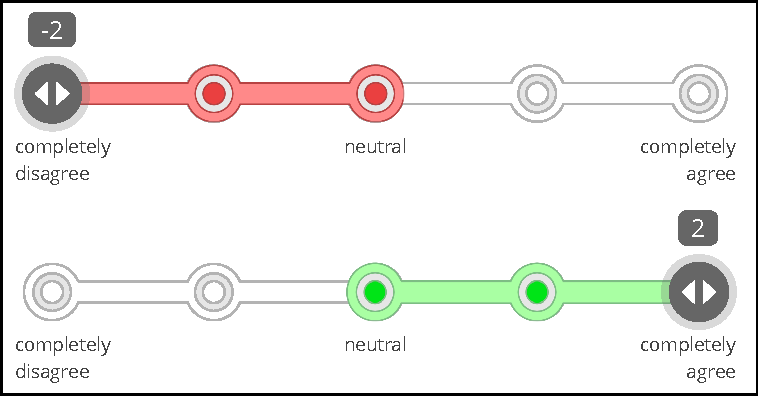
\includegraphics[width=10cm]{slikert}
\end{exampleResultBox}

\vspace{1cm}

\subsection{test variable}\label{subsec:test-variable}

A test variable allows to inject some data into a page which is dependant on the test it's found in.
For instance if you use a default welcome page, that only changes the title each time to reflect what test this is.

Instead of creating 20 copies of the same content page with a different title each time—which is really stressful if you decide to make a change to the text, and need to do it 20 time over—you can create one page which uses a test variable as title.
The appropriate text to inject here is then set in the test manager for each test. \\

Syntax:\hspace{0.5cm}\kw{[@VAR ... @]}

\begin{properties}
\hline
NAME & the name of the variable to insert here—this must match the name given in the test manager\\
\hline
\end{properties}
\vspace{0.1cm}

\begin{exampleBox}{Example}
	The title of a test could look like this:\\
	\kw{[@VAR NAME="testtitle"@]}
\end{exampleBox}

\begin{advancedBox}{Advanced tip}
	Instead of defining the variable contents in the test manager, it can also be sent with a GET parameter called "variables" to the index.php of OASYS (usually sent together with login and password for direct login):\\ 
	
	\kwp{variables = "\{testtitle: \{global: true, text: \{EN: 'Mathematics Intermediate'\}\}\}"} \\
	
		In this example we do not want different strings per language, so the \kwp{global} is set to \kwp{true}.
		This means it will take the first and only defined language (EN in this case) and use it for all languages. \\
	
	The variable must be transmitted in JSON encoded format as shown above.
	
\end{advancedBox}

ATTENTION: this keyword is deprecated as of OASYS 3.6.0. The new way to do this is to use the syntax \kw{\{\{variableName\}\}} instead, which allows this to be used in any text to be displayed, no matter which interaction is used. An advanced editor interaction is no longer required for this. \\

\subsection{test index}\label{subsec:test-index}

The test index keyword automatically creates an index of all stimuli in a test with a link to navigate to them directly.
The main use for this is for literature tests where you will have several test pages sharing the same stimulus and a new question about the stimulus on every page. \\

The test index, which would be put on a separate page at the beginning, will enumerate all stimuli with their name as defined in the content manager and let the user navigate to the first occurrence of each piece of literature.
Pages without a stimulus will be ignored by default, but this behaviour can be configured with an attribute.

Syntax:\hspace{0.5cm}\kw{[@INDEX ... @]}

\begin{properties}
\hline
ALL & if present (no value needed) this attribute forces the index to also show standalone pages that do not have a stimulus—by default this is off\\
\hline
\end{properties}
\vspace{0.1cm}

\begin{exampleBox}{Example}
	A test index that shows standalone pages as well as stimuli:\\
	\kw{[@INDEX ALL@]}
\end{exampleBox}

\subsection{link}\label{subsec:link}

Links are keywords that are put around a label or piece of text in order to make it clickable for navigation purposes.
Their main purpose is to combine them with an overview of given answers and allow the test taker to navigate back in order to make changes.
They can navigate forward as well as backward as long as the target is found in the test structure.

Syntax:\hspace{0.5cm}\kw{[@LINK ... @]}label of the link\kw{[@/LINK@]}

\begin{properties}
\hline
FIRST & if present (no value needed), this links to the first page in the structure\\
LAST & if present (no value needed), this links to the last page in the structure\\
CODE & this links to the page with the indicated item code no matter where it is found in the test structure \\
PAGE & this links to the indicated page (integer value) starting count at 1 up to the number of pages in the structure.
This method will cause trouble when the test structure is changed, so targeting with the item code is generally a better choice.
If this value is "-1" then it is a synonym of the \kw{LAST} attribute. \\
RELATIVE & this links to another page relative to the current position.
For instance "+2" would skip ahead 2 pages while "-1" would mean you go back to the previous page. \\
\hline
\end{properties}
\vspace{0.1cm}

\begin{exampleBox}{Example}
	Skip ahead 5 pages:\\
	\kw{[@LINK RELATIVE="+5"@]}cut to the chase\kw{[@/LINK@]}
\end{exampleBox}

\subsection{overview}\label{subsec:overview}

The overview shows information about answers given in previous pages.
It is used as a summary of sorts to be presented at the end of a test.
It can also be used to show the contents of some internal variables, although those are generally used in scripting and displaying them is not very useful for the test taker. For a list of defined variables, please refer to the scripting documentation. \\
Overview elements can take various shapes depending on the format of the data.

Syntax:\hspace{0.5cm}\kw{[@OVERVIEW ... @]}

\begin{properties}
\hline
TYPE & this defines the visual form of the overview.
The allowed values are: \kw{checkmark}, \kw{value}, \kw{list}, \kw{progress}\\
& \kw{checkmark} will simply show a checkmark if a response has been given to the indicated field; if a boolean variable is displayed it shows a checkmark for true and a red X for false \\
& \kw{value} shows the actual answer as is (useful primarily if the answer is a number or a short string) \\
& \kw{list} shows a predefined answer from a list based on a numerical answer \\
& \kw{progress} shows a small progress bar which is based on a numerical answer—behind the progress bar the actual value is also shown as text\\
SOURCE & indicates the name of the variable to base overview on \\
COLOUR & CSS colour string in which to render the overview—default is "\#000000" (black) \\
MIN & the minimum number a numerical answer can take [only for \kw{list} type and \kw{progress} type]—this number can be a decimal number (positive or negative)\\
MAX & the maximum expected number from a numerical source (c.f. \kw{MIN} for further details) \\
WIDTH & the width for a \kw{progress} bar in CSS units—default is 50px \\
HEIGHT & the height for a \kw{progress} bar in CSS units—default is 0.5em \\
FONTSIZE & the font size to use for any text output (applies to \kw{checkmark}, \kw{value}, \kw{list} and the label next to a \kw{progress} bar)—default is 1em \\
LIST & a list of labels to show depending on a numerical answer.
The answers are separated by pipe symbols (|).
If \kw{MIN} has been set to -2 the first label will be displayed for the value of -2, the second for -1, etc. \\
& If the expected numbers do not increase by 1, the values need to be specified with the labels.
For instance if we are expecting -4, -2, 0, 2 and 4 as values the list might look like this: \textit{"-4: strongly disagree|-2: disagree|0: neutral|2: agree|4: strongly agree"}\\
HIDELABEL & this applies only to \kw{progress} type and will hide the full text answer next to the progress bar\\
\hline
\end{properties}
\vspace{0.1cm}

\begin{exampleBox}{Example}
	A progress bar that gets data from a \kw{slikert} which exports under the name "Q01" and has a scale from 1 to 7:\\
	\kw{[@OVERVIEW COLOUR="\#52B6E0" TYPE="progress" SOURCE="Q01" MIN="1" MAX="7"@]} \\
	
	And here we have data from a radio button group (exporting under the name Q14) which can take values 1 or 2 representing "yes" or "no":\\
	\kw{[@OVERVIEW COLOUR="\#52B6E0" TYPE="list" SOURCE="Q14" MIN="1" LIST="Yes|No"]}
\end{exampleBox}


\subsection{local timer}\label{subsec:local-timer}

This creates a countdown for the currently shown page.
When the timer reaches zero the test taker will be automatically navigated to the next page.
It is also possible to link a few pages in order to create a countdown for a block of pages. \\

Syntax:\hspace{0.5cm}\kw{[@TIMER@]} \\

\begin{properties}
\hline
ID & this defines a name for the timer—by using the same name on several consecutive pages those pages are grouped together in the same timer and the whole block of pages is skipped when the countdown hits zero\\
TIMEOUT & the time of the countdown in seconds \\
\hline
\end{properties}
\vspace{0.1cm}

\begin{exampleBox}{Example}
	A 2 minute countdown:\\
	\kw{[@TIMER ID="block01" TIMEOUT="120"@]}
\end{exampleBox}

\begin{advancedBox}{Notes}
	\begin{itemize}
		\item This keyword must be put into a paragraph by its own.
		The paragraph will be removed completely when rendering the page.
		\item The \kwp{ID} must not be "default" which is a reserved identifier for internal use
		\item The local timer requires the test to limit navigation, so that the test taker can never go backwards	
		\item The test must not have a global timer for the whole test—if it does, the local timers are ignored
		\end{itemize}
\end{advancedBox}

\subsection{button}\label{subsec:button}

Syntax:\hspace{0.5cm}\kw{[@BUTTON ... @]}

\begin{properties}
\hline
LABEL & the text to be visible on the button \\
NAME & same as \kw{LABEL}—deprecated (for backwards compatibility) \\
ACTION & an action out of a predefined list to be executed on pressing the button \\
FUNCTION & same as \kw{ACTION}—deprecated (for backwards compatibility) \\
\hline
\end{properties}
\vspace{0.1cm}

List of defined actions:

\begin{properties}
\hline
endTest & ends a test as if the time was up.
If there is another test attached to this pair of credentials that will be loaded, otherwise the login resp.
landing page will be loaded or the score will be shown if the test was so configured \\
gotoLogin & takes the user back to the login resp.
landing page, no matter if another test was attached to the currect pair of credentials.
Also the test that was aborted will not be closed, so that it can be logged into again at a later time \\
nextPage & this takes the user to the next page even if conditions are not met (if limit naviagtion is enabled in the test) \\
previousPage & this takes the user back to the previous page, even if the navigation limit is enabled and moving backwards is not allowed \\
\hline
\end{properties}
\vspace{0.1cm}

\begin{exampleBox}{Example}
	A typical button to close the test (necessary if there is no test timer):\\
	\kw{[@BUTTON LABEL="Close test" ACTION="endTest"@]}
\end{exampleBox}

Note: due to backwards compatibility with OASYS v1.0 content, the actions are sometimes found with a set of brackets which may or may not contain paramaters.
Those parameters are not evaluated by OASYS v3.x, but might be in a future version. \\
Thus if you see the attribute \kw{FUNCTION="endTest()"}, that is identical to \kw{ACTION="endTest"}.\\

\subsection{css rule}\label{subsec:css-rule}

Syntax:\hspace{0.5cm}\kw{[@CSS ... @]}

\begin{properties}
\hline
SELECTOR & a CSS selector as standardized by w3.org\\
RULES & standard CSS rules separated with semicolons \\
\hline
\end{properties}
\vspace{0.1cm}

\begin{exampleBox}{Example}
	Defining the padding of all table cells on page:\\
	\kw{[@CSS SELECTOR="table tr > td" RULES="padding: 10px 5px;"@]}
\end{exampleBox}

\begin{advancedBox}{Notes}
This keyword must be put into a paragraph by its own.
The paragraph will be removed completely when rendering the page.
\end{advancedBox}

\subsection{drag and drop}\label{subsec:drag-and-drop}

In order to create a drag and drop item two elements are necessary: a draggable than can be moved by the test taker and a dropzone where the draggable can be docked.
Every dropzone represents a variable in the results of a test and it will contain the value of the draggable docked into it.
Dropzones that can accept more than a single draggable will report a JSON array of values docked in it. \\

If some draggables should only be able to be dropped on a specific dropzone and other on another dropzone, we can define a group for a draggable and a list of groups accepted by a dropzone.

Syntax of a draggable:\hspace{0.5cm}\kw{[@DG ... @]}

\begin{properties}
\hline
VALUE & this is the value reported back by the dropzone in which this draggable has been dropped.
Since values designate the different draggables, they need to be within a page \\
GROUP & an optional group which allows a dropzone to decide if it can accept this draggable or not \\
IMAGE & the url of an image to show inside the draggable \\
LABEL & a text label to show inside the draggable (only if not using \kw{IMAGE} attribute—may contain HTML tags like <b>, <i> … etc. \\
STYLE & CSS string to apply to draggable, different rules can be separated by semicolons \\
CLONE & if value is non zero, this attribute makes a stencil out of a draggable—instead of moving the draggable a copy of it will be created and moved.
The number of existing copies is only limited by the available space to drop them. Dropzones must be configured to accept clones for this to work. \\
\hline
\end{properties}
\vspace{0.1cm}

Syntax of a dropzone:\hspace{0.5cm}\kw{[@DZ ... @]}

\begin{properties}
\hline
ID & his defines the variable name for the results of the dropzone;
if omitted, the fields will be autonamed: dnd\_1, dnd\_2, \ldots etc. \\
ACCEPTCLONES & if present the dropzone will allow clones to dock there, and only clones \\
GROUPS & a list of groups to accept in this dropzone (c.f. \kw{GROUP} attribute of draggables—if more than 1 group the names must be delimited by pipe symbols\\
IMAGE & the url of an image to show inside the dropzone \\
LABEL & a text label to show inside the dropzone (only if not using \kw{IMAGE} attribute—may contain HTML code\\
STYLE & CSS string to apply to dropzone, different rules can be separated by semicolons \\
TYPE & either \kw{default} or \kw{remove}, whereas the latter is used to create a trashcan for draggable clones—if omitted the dropzone defaults to a normal behaviour. As of OASYS 3.6.0 the type \kw{remove} now implies \kw{ACCEPTCLONES}. \\
ONFULL & either \kw{replace} to kick the previous occupant of this dropzone out to accept a new one or \kw{refuse} to refuse new draggables if there is no more space for them \\
MAX & the count of slots available in the dropzone to accept draggables—default is 1 \\
PADDING & number of pixels to leave between border and the position of the draggable being docked—due to technical reasons padding must be specified with this attribute instead of the \kw{STYLE} attribute—if given 1 value it will be applied for all sides, if given 2 values the first is for top and bottom and the second for left and right and if 4 values are given it will be assigned in the order: top, right, bottom, left \\
ZINDEX & the CSS z-index value for docked draggables—by default it's 1 and it only needs to be increased if the dropzone itself has a higher z-index than 0 \\
ORIENTATION & only for dropzones that accept more than 1 draggable: \kw{vertical} or \kw{horizontal} to decide how to orient the docked objects \\
ALIGNMENT & only for dropzones that accept more than 1 draggable: by default the objects are arranged from left to right on horizontal orientation and top to bottom for vertical orientation.
To change this write either \kw{right} resp. \kw{bottom} into this attribute to go from right to left resp.
from bottom to top. \\
SPACING & only for dropzones that accept more than 1 draggable: space in number of pixels to leave between 2 draggables when docking—default is 5 pixels \\
GRID &  only for dropzones that accept more than 1 draggable: while normally every draggable gets the size it needs, it is also possible to define a fixed size for a grid (number of pixels) in order to dock objects evenly ignoring their size.
If the draggables are larger than the space allotted to them, they will overlap. \\
ONDROP & for dropzones that accept more than 1 draggable there are 4 different configurations to decide where to place a dropped draggable when the dropzone already contains others: \\
& \kw{beginning}: every new draggable is docked in front of the previous ones (that would be left if a dropzone is horizontally oriented and aligned to the left, but it would be on the right for horizontal orientation with right alignment, and similar for the vertically oriented dropzones)—this is the default setting \\
& \kw{end}: every draggable is added at the end of the list, again depending on the orientation and alignment \\
& \kw{insert}: the draggable is insert at the place where it is dropped.
In this case it is also possible to rearrange the order of draggables inside the dropzone by dragging them to a different position \\
& \kw{auto}: the draggables are ordered automatically by a value given to it (check out the \kw{ORDERBY} attribute below) \\
ORDERBY &  only for dropzones that have the \kw{ONDROP} attribute set to \kw{auto}: currently this can only to be set to \kw{value} in order to arrange draggables automatically by their value [other configuration options to come in future versions of OASYS] \\
CONTAINS & a list of values of the draggables contained in this dropzone at creation time—if more than one draggable, values need to be separated by pipe symbols.
If all available draggables are to start off here set this to "*"\\
RULE & in order to satisfy requirements for a drag and drop item and allow the test taker to proceed to next page (if limit navigation is enabled in the test) it is imperative to define what is expected.
If we require a dropzone to get exactly 1 draggable its rule will have to be "1", if we expected it to contain 1 or more we set the rule to "1+" or ">0".
If we expect 3 or less the rule will be "3-" or "<4".
Last but not least if we want 2, 3 or 4 draggables in a dropzone the rule has to be "2..4". \\
\hline
\end{properties}
\vspace{0.1cm}

\begin{exampleBox}{Example}
	An example where 4 draggables must be dragged to 4 different dropzones (which would be accompanied by images not represented here).
	All draggables start out in the dropzone called "stock" which is expected to be empty at the end, hence its RULE="0":\\

\footnotesize

\kw{[@DG ID="dg01" STYLE="width: 60px; height: 25px; border: 1px solid; padding: 10px; background-color: \#E5F2F7; text-align:center;" VALUE="1" LABEL="10 cm" @]}\\
\kw{[@DG ID="dg02" STYLE="width: 60px; height: 25px; border: 1px solid; padding: 10px; background-color: \#E5F2F7; text-align:center;" VALUE="2" LABEL="4 dm" @]}\\
\kw{[@DG ID="dg03" STYLE="width: 60px; height: 25px; border: 1px solid; padding: 10px; background-color: \#E5F2F7; text-align:center;" VALUE="3" LABEL="300 cm"@]}\\
\kw{[@DG ID="dg04" STYLE="width: 60px; height: 25px; border: 1px solid; padding: 10px; background-color: \#E5F2F7; text-align:center;" VALUE="4" LABEL="7 m"@]}\\

\kw{[@DZ ID="dz01" STYLE="width: 80px; height: 45px; background-color: \#eeeeee; border: 1px solid black;" @]}\\
\kw{[@DZ ID="dz02" STYLE="width: 80px; height: 45px; background-color: \#eeeeee; border: 1px solid black;" @]}\\
\kw{[@DZ ID="dz03" STYLE="width: 80px; height: 45px; background-color: \#eeeeee; border: 1px solid black;" @]}\\
\kw{[@DZ ID="dz04" STYLE="width: 80px; height: 45px; background-color: \#eeeeee; border: 1px solid black;" @]}\\

\kw{[@DZ ID="stock" CONTAINS="*" RULE="0" MAX="4" ORIENTATION="horizontal" STYLE="width: 356px; height: 60px; border: 1px solid black;" PADDING="7"@]}

\end{exampleBox}
\vspace{0.1cm}

\begin{advancedBox}{Notes}
The \kwp{[@DG … @]} keyword must be put into a paragraph by its own.
The paragraph will be removed completely when rendering the page.
The \kwp{[@DZ … @]} keyword must be place in context where the dropzone is to be created.
\end{advancedBox}

%\subsection{xxx}
%
%Syntax:\hspace{0.5cm}\kw{[@XX ... @]}
%
%\begin{properties}
%\hline
%ID & this defines the variable name for the results of the XXX; if omitted, the fields will be autonamed: XX\_1, XX\_2, ... etc.\\
%\hline
%\end{properties}
%\vspace{0.1cm}
%
%\begin{exampleBox}{Example}
%	xxx:\\
%	\kw{[@XXX …@]}
%\end{exampleBox}

\section{Using formulas in OASYS}\label{sec:using-formulas-in-oasys}

In OASYS it is possible to use mathematical formulas.
This is possible in any editor that allows text entry (e.g.\ labels, etc.).\\

In order to add a formula OASYS uses \LaTeX.
There are 2 ways to use \LaTeX in OASYS: as an inline formula or as a standalone line centered on the screen.\\

To write a formula inline the \LaTeX text is written between the starting and closing tags \kw{[\$} and \kw{\$]}.
To use a complete line use the tags \kw{[\$\$} and \kw{\$\$]} instead.\\

There is one exception however, where the tags with the square brackets will not work: in an inline type interaction, like the "inline gaps", it is impossible to use this syntax inside a gap, since there would be a conflict as the gap keywords do not allow square brackets. For this reason a set of alternative tags were introduced in OASYS v3.5.31, while the above syntax will continue to be supported throughout OASYS as well. The alternative tags are \kw{\{\$} and \kw{\$\}}, respectively \kw{\{\$\$} and \kw{\$\$\}}.\\

\begin{exampleResultBox}{Example of inline mode:}
What will be the result of [\$x\^\@y\$] if x=4 and y=2?
\tcblower
\tcbsubtitle{This will be rendered afterwards like this:}
What will be the result of $x^y$ if x=4 and y=2?
\end{exampleResultBox}

\vspace{1cm}

\begin{exampleResultBox}{Example of full line:}
[\$\$\textbackslash frac\{x\}\{y\} = ?\$\$]
\tcblower
\tcbsubtitle{This will be rendered afterwards like this:}
\[\frac{x}{y} = ?\]
\end{exampleResultBox}

\end{document}



